\chapter{Background and related work}

\section{Language, social Identity and stereotyping}

\textbf{Background}
\begin{itemize}
    \item Origin of bias (System -1 and system -2) ; TWO FAMILIES OF COGNITIVE OPERATIONS \cite{kahneman2002representativeness}
    \item  How stereotypes are inevitably formed (implicit bias) ??
    Impressions + labels ...
    \cite{fiske1998stereotyping}
    \item Difference between stereotype and prejudice \cite{fiske1998stereotyping}
\end{itemize}
\textbf{Perspectives of stereotypes}
\begin{itemize}
    \item Describe two perspective, Stereotypes as pictures in head and stereotyping (shared social beliefs and expectencies) 
    \item Definitions of stereotype from other papers
    \item Cognitive processes in stereotyping and intergroup behavior \cite{hamilton2015cognitive}
    \item Stereotypes and stereotyping \cite{macrae1996stereotypes}
    \item Representational harms caused by stereotypes [Kate Crawford. 2017. The Trouble with Bias. Keynote
at NeurIPS]
\end{itemize}
\textbf{How language contributes to stereotype formation}
    \begin{itemize}
        \item Stereotypes as collective belief systems \cite{macrae1996stereotypes}
        \item How language contributes to stereotype formation \cite{burgers2020language}
        \item How stereotypes are shared through language: a
    review and introduction of the social categories
    and stereotypes communication (SCSC) framework \cite{beukeboom2019stereotypes}
    \end{itemize}
\section{Machine learning and deep learning}
\subsection{Machine learning pipeline}
    \begin{itemize}
        \item Machine learning setup by abu mustafa 
        \begin{figure}[t]
            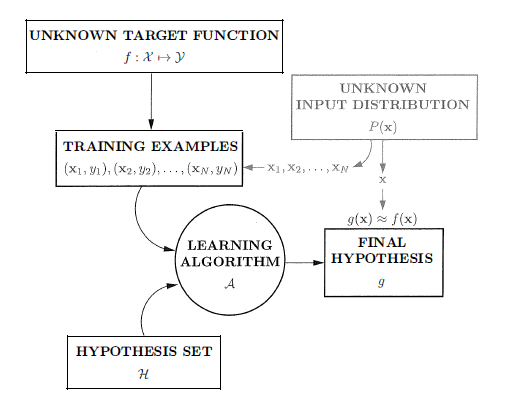
\includegraphics[width=8cm]{thesis/figures/Learning problem.PNG}
            \centering
            \caption{The learning problem setup}
            \label{fig:The learning problem setup}
        \end{figure}
        \begin{enumerate}
            \item Explain different components of learning problem  learning problem 
            
        \end{enumerate}
        \item Types of training (supervised, unsupervised, reinforcement learning and focus on supervised)
        \item Learning models (Classification, regression)
        \item Linear Regression and gradient descent 
        % \item SVM and selected classifiers \textbf{TBD ??}
    \end{itemize}
\subsection{Neural Networks architecture}
    \begin{itemize}
        \item Neural network basic setup (perceptron learning algorithm)
        \item Basic neural network forward pass and backward pass
        \item  Deep neural network and its variants
    \end{itemize}
\subsection { Recurrent Neural Networks }
            \begin{itemize}
                \item Limitations of NN 
                \item Why RNN when dealing with text ?
                \item Contextual word embedding
            \end{itemize}

\subsection{Transformer architecture}
    
\section{Natural language processing and language modeling}
    \subsection{Vector representation of language}
    \begin{itemize}
        \item What is NLP?
        \item Feature vectors for text 
        \item Word embeddings
        \item Static word embedding
        \item Word2vec, glove basic architecture
    \end{itemize}
    \subsection{Language modeling}
    \subsection{Transfer learning}
    \subsection{BERT architecture}
\section {Evaluation metrics}    
\section{Bias and social bias in Natural language processing}
\begin{itemize}
    \item A critical survey of bias in NLP \cite{blodgett2020language}
    \item A survey on Bias in Deep NLP \cite{garrido2021survey}
\end{itemize}